%%%%%%%%%%%%%%%%%%%%%%%%%%%%%%%%%%%%%%%%%%%%%%%%%%%%%%%%%%%%%%%%%%%%%%%%%%%%%%%%%%%%%%%%%%%%%%%%%%%%%
% \begin{frame}{Outline1}
% \begin{itemize}
%  \item \ldots
% \end{itemize}
% \end{frame}


 
\begin{frame}{Outline}
\footnotesize
\begin{itemize}
\item What is Synthetic Biology?
\item How to computationally design "improved" proteins
\item What are the challenges for Computational chemistry?
\end{itemize}
\end{frame}


\begin{frame}{Outline}
\footnotesize

\begin{itemize}
\item \textbf{What is Synthetic Biology?}
\begin{itemize}
\item Objectives and Foundations
\item History of Cells
\item Steps for synthetising new proteins 
\item Challenges of synthetic biology
\end{itemize}
\item How to computationally design "improved" proteins
\item What are the challenges for Computational chemistry?
\end{itemize}
\end{frame}

%%%%%%%%%%%%%%%%%%%%%%%%%%%%%%%%%%%%%%%%%%%%%%%%%%%%%%%%%%%%%%%%%%%%%%%%%%%%%%%%%%%%%%%%%%%%%%%%%%%%%
\begin{frame}{What is Synthetic Biology?}
\footnotesize

\begin{itemize}
\item \textbf{Goals}: 
\begin{itemize}
\footnotesize
\item \textbf{To produce new biological systems to carry out some desired and well-defined functions}
\item To develop an engineering technology for the living systems (faster, cheaper, more efficient for a wide usage of engineering principles)
\end{itemize}
\item \textbf{How?}
\begin{enumerate}
\footnotesize
\item by designing a new protein structure fitting the needs
\item by generating DNA sequences that fold to the desired structure
\item by introducing this synthetic DNA in a cell that will process it
\end{enumerate}

\item a recent scientific field \\

\begin{columns}[c] % the "c" option specifies center vertical alignment
\column{.4\textwidth} % column designated by a command

\column{.6\textwidth}
\setlength\fboxsep{0pt}
\setlength\fboxrule{0.5pt}
\fbox{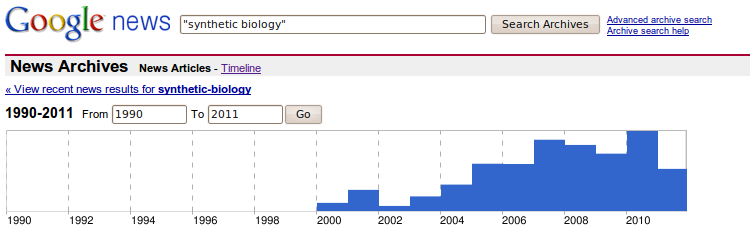
\includegraphics[width=1.0\textwidth]{./images/GoogleSynBio.png}}
\end{columns}

\end{itemize}
\end{frame}

%%%%%%%%%%%%%%%%%%%%%%%%%%%%%%%%%%%%%%%%%%%%%%%%%%%%%%%%%%%%%%%%%%%%%%%%%%%%%%%%%%%%%%%%%%%%%%%%%%%%%
\begin{frame}{Analogy to Computer Engineering}
\footnotesize
Foundations:
\begin{itemize}
\footnotesize
\item "Cells are processors"
\item "DNA is a (low-level) programming language"
\end{itemize}
\begin{center}
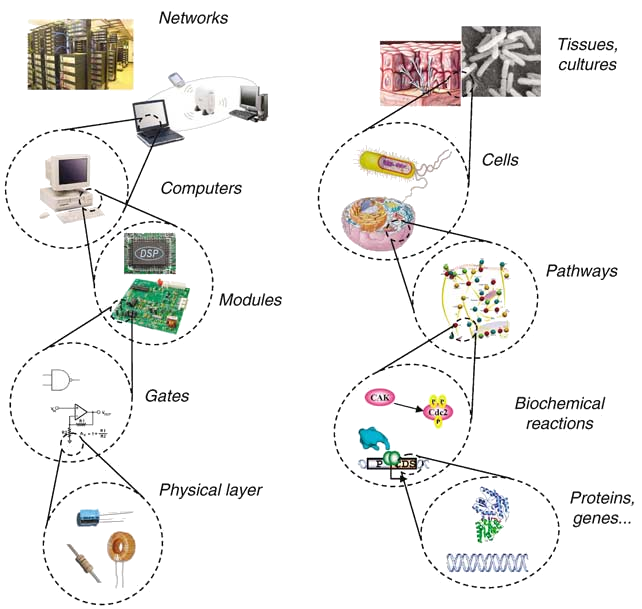
\includegraphics[width=0.7\textwidth]{./images/SynBio_ComputerEngineering.png} 
\end{center}
%   \begin{reference}{15mm}{85mm}
%   Andrianantoandro, E. et al. Synthetic biology: new engineering rules for an emerging discipline.
% Molecular systems biology 2, 2006.0028(2006).
%    \end{reference} 

\end{frame}
%%%%%%%%%%%%%%%%%%%%%%%%%%%%%%%%%%%%%%%%%%%%%%%%%%%%%%%%%%%%%%%%%%%%%%%%%%%%%%%%%%%%%%%%%%%%%%%%%%%%%
\begin{frame}{Computing vs Genetics}
\footnotesize
\begin{center}
\begin{tabular}{c | c}
        Digital code  & A T G C \\ \hline
        Open standards & (e.g. codons) \\ \hline
        Modular code  & Genes\\ \hline
        Error protection  & DNA repair\\ \hline
        Data compression  & Overlapping ORFs\\ \hline
        Redundant backups  & Double helix, Copy number\\ \hline
        Self diagnostics & Apoptosis\\ \hline
        Firewalls & Species\\ \hline
        Operating systems & Ribsomes\\ 
\end{tabular}
\end{center}

\end{frame}
%%%%%%%%%%%%%%%%%%%%%%%%%%%%%%%%%%%%%%%%%%%%%%%%%%%%%%%%%%%%%%%%%%%%%%%%%%%%%%%%%%%%%%%%%%%%%%%%%%%%%
\begin{frame}{History of Cells - Theory of Evolution (1859)}
\footnotesize
\begin{center}
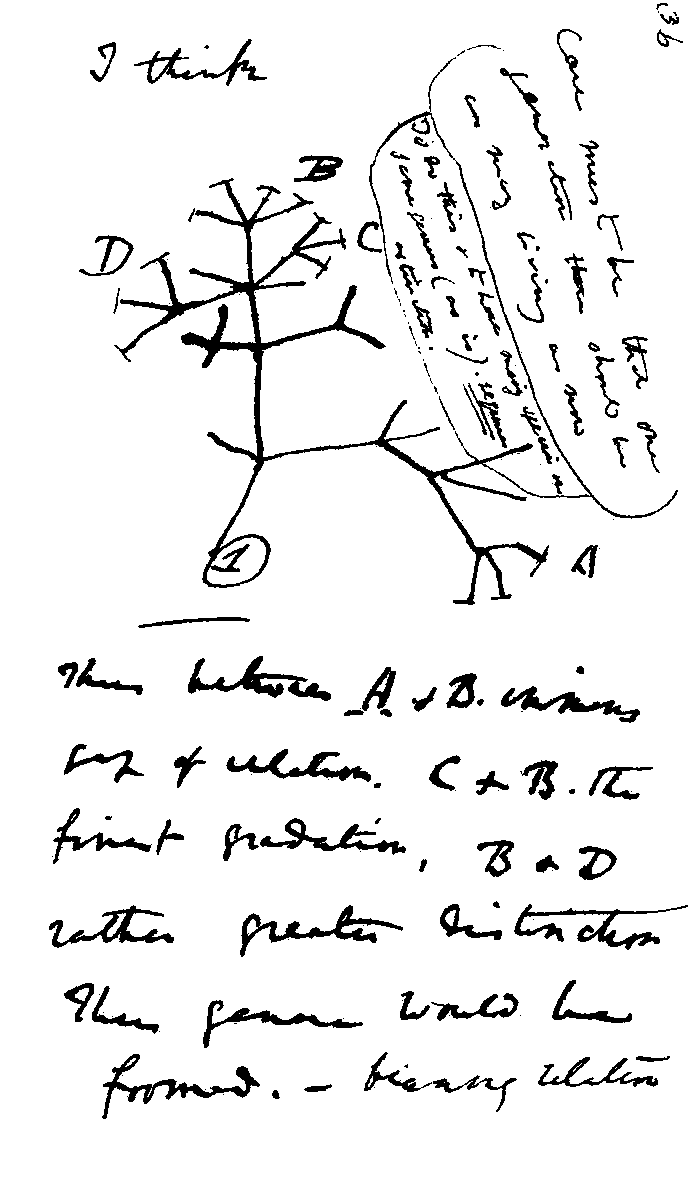
\includegraphics[width=0.45\textwidth]{./images/Darwin_tree.png} 
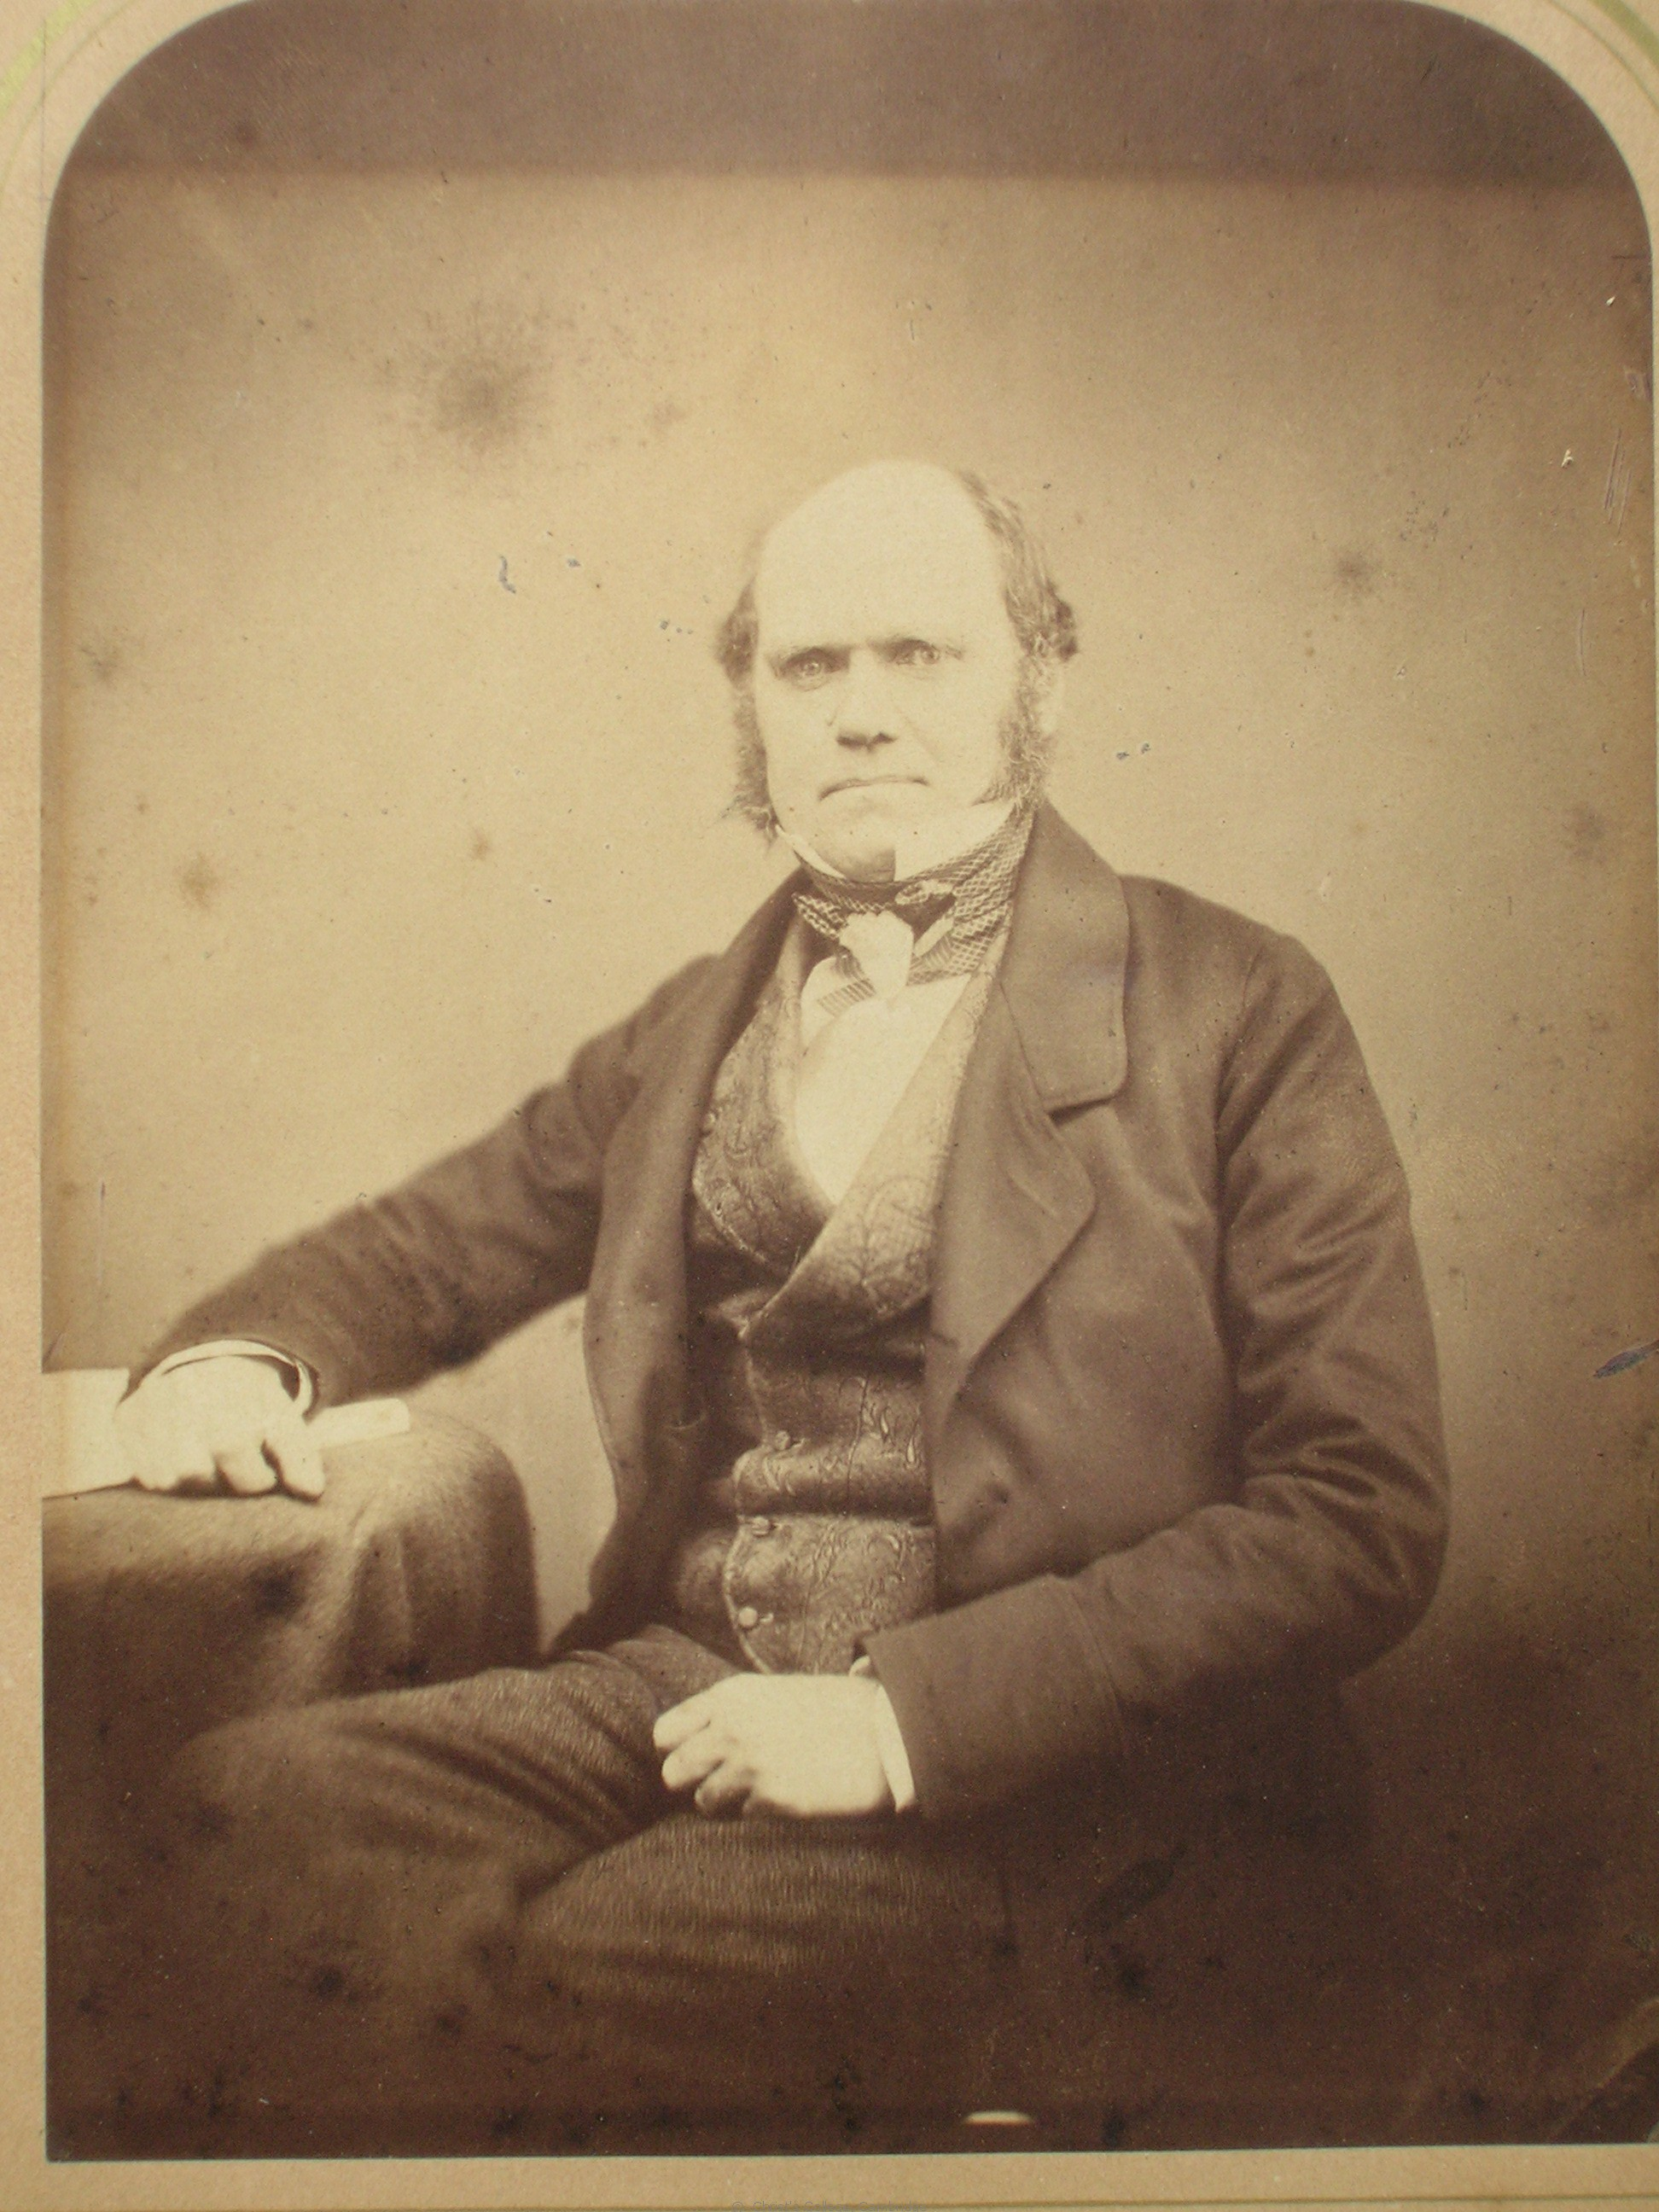
\includegraphics[width=0.5\textwidth]{./images/darwin-1855_photo.jpg} 
\end{center}
\end{frame}

%%%%%%%%%%%%%%%%%%%%%%%%%%%%%%%%%%%%%%%%%%%%%%%%%%%%%%%%%%%%%%%%%%%%%%%%%%%%%%%%%%%%%%%%%%%%%%%%%%%%%
\begin{frame}{History of Cells - DNA Structure (1953)}
\footnotesize
\begin{center}
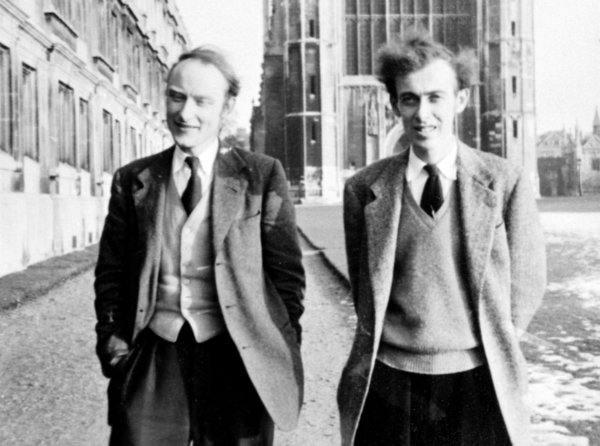
\includegraphics[width=0.7\textwidth]{./images/portrait-wcwalking-600w.jpg} 
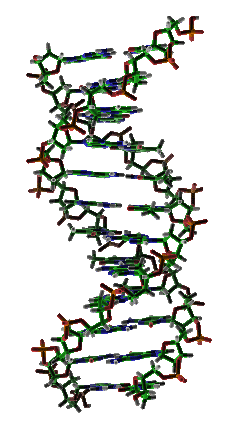
\includegraphics[width=0.3\textwidth]{./images/DNA_orbit_animated_static_thumb2.png} 
\end{center}
\end{frame}

%%%%%%%%%%%%%%%%%%%%%%%%%%%%%%%%%%%%%%%%%%%%%%%%%%%%%%%%%%%%%%%%%%%%%%%%%%%%%%%%%%%%%%%%%%%%%%%%%%%%%
\begin{frame}{History of Cells - DNA mapping to proteins}
\footnotesize
\begin{center}
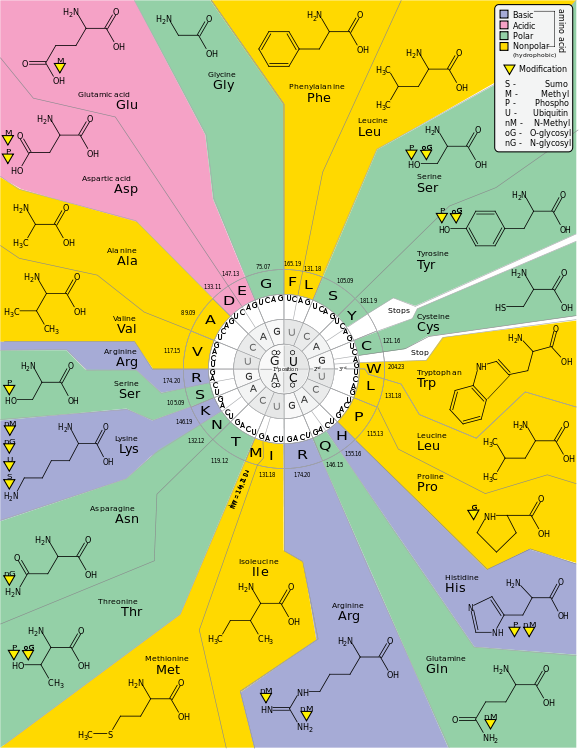
\includegraphics[width=0.55\textwidth]{./images/GeneticCode21-version-2.png} 
\end{center}
% 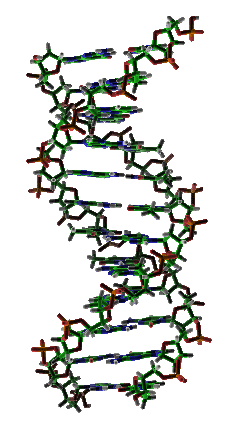
\includegraphics[width=0.3\textwidth]{./images/DNA_orbit_animated_static_thumb.png} 
\end{frame}

%%%%%%%%%%%%%%%%%%%%%%%%%%%%%%%%%%%%%%%%%%%%%%%%%%%%%%%%%%%%%%%%%%%%%%%%%%%%%%%%%%%%%%%%%%%%%%%%%%%%%
\begin{frame}{How to work with it?}
\footnotesize

 
\begin{itemize}
\item READING
\item COMPREHENSION
\item WRITING
\end{itemize} 
\end{frame}

%%%%%%%%%%%%%%%%%%%%%%%%%%%%%%%%%%%%%%%%%%%%%%%%%%%%%%%%%%%%%%%%%%%%%%%%%%%%%%%%%%%%%%%%%%%%%%%%%%%%%
\begin{frame}{Reading DNA}
\footnotesize

    \begin{columns}[c] % the "c" option specifies center vertical alignment
      \column{.5\textwidth} % column designated by a command
\begin{itemize}
\item in the 70's: dangerous and $<500bp/day$
\item Few numbers:
  \begin{itemize}
\footnotesize
  \item e-Coli bacteria: 5 Mega base-pairs (bp), compact powerful $\sim 5000$ genes
  \item human: 6000Mbp, $\sim 25000$ genes
  \end{itemize} 
\item since 1998, Automated sequencer: $\sim 0.5Mbp/day$
\item impressive growth of genBank (1981 to 2008)
\end{itemize} 
      \column{.5\textwidth}
      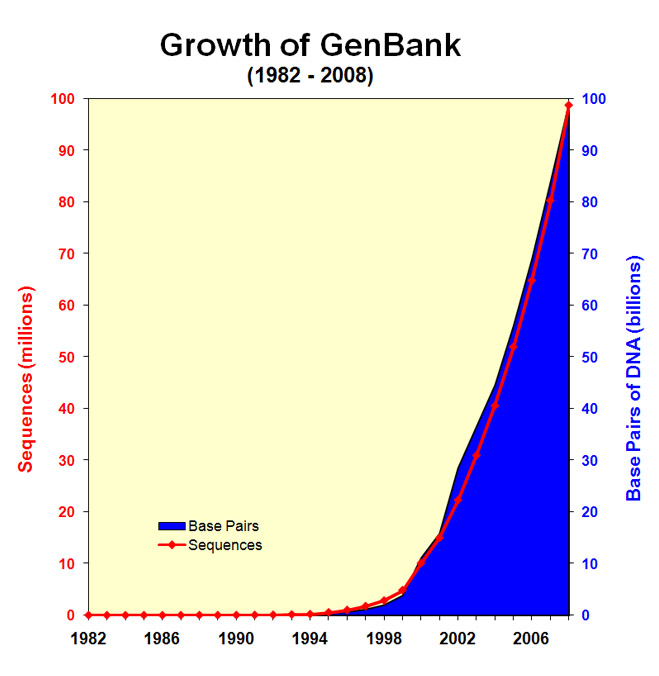
\includegraphics[width=1.0\textwidth]{./images/genbankgrowth.jpg} 
    \end{columns}
\end{frame}
%%%%%%%%%%%%%%%%%%%%%%%%%%%%%%%%%%%%%%%%%%%%%%%%%%%%%%%%%%%%%%%%%%%%%%%%%%%%%%%%%%%%%%%%%%%%%%%%%%%%%
\begin{frame}{Comprehension of DNA}
\footnotesize
    \begin{columns}[c] % the "c" option specifies center vertical alignment
      \column{.5\textwidth} % column designated by a command
      \begin{itemize}
      \item They can make \textbf{a whole bacterial genomic map}
% %       \item They can sequence species ($>5000$ species decoded and listed in \textbf{GenBank})
% %       \item They can show \textbf{relationship between proteins} of a system (e-Coli)
% % % % %       \item They can generate the 3D shape of a protein (fold.It)
      \end{itemize} 
  
      \column{.5\textwidth}
    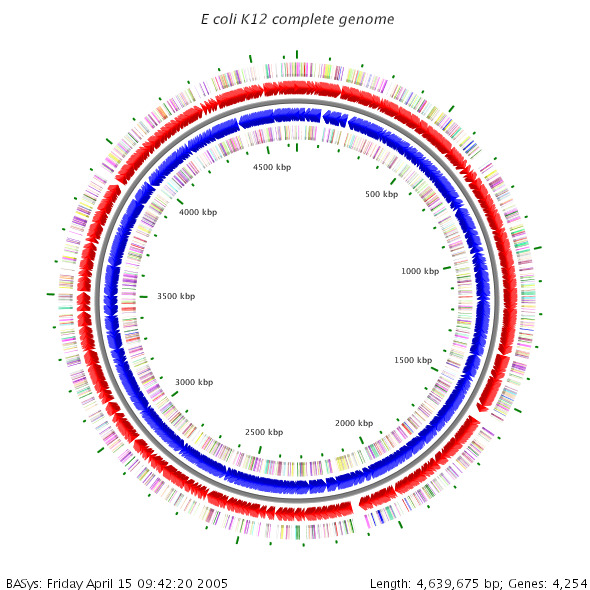
\includegraphics[width=1.2\textwidth]{./images/BABsys2.png} 			
%     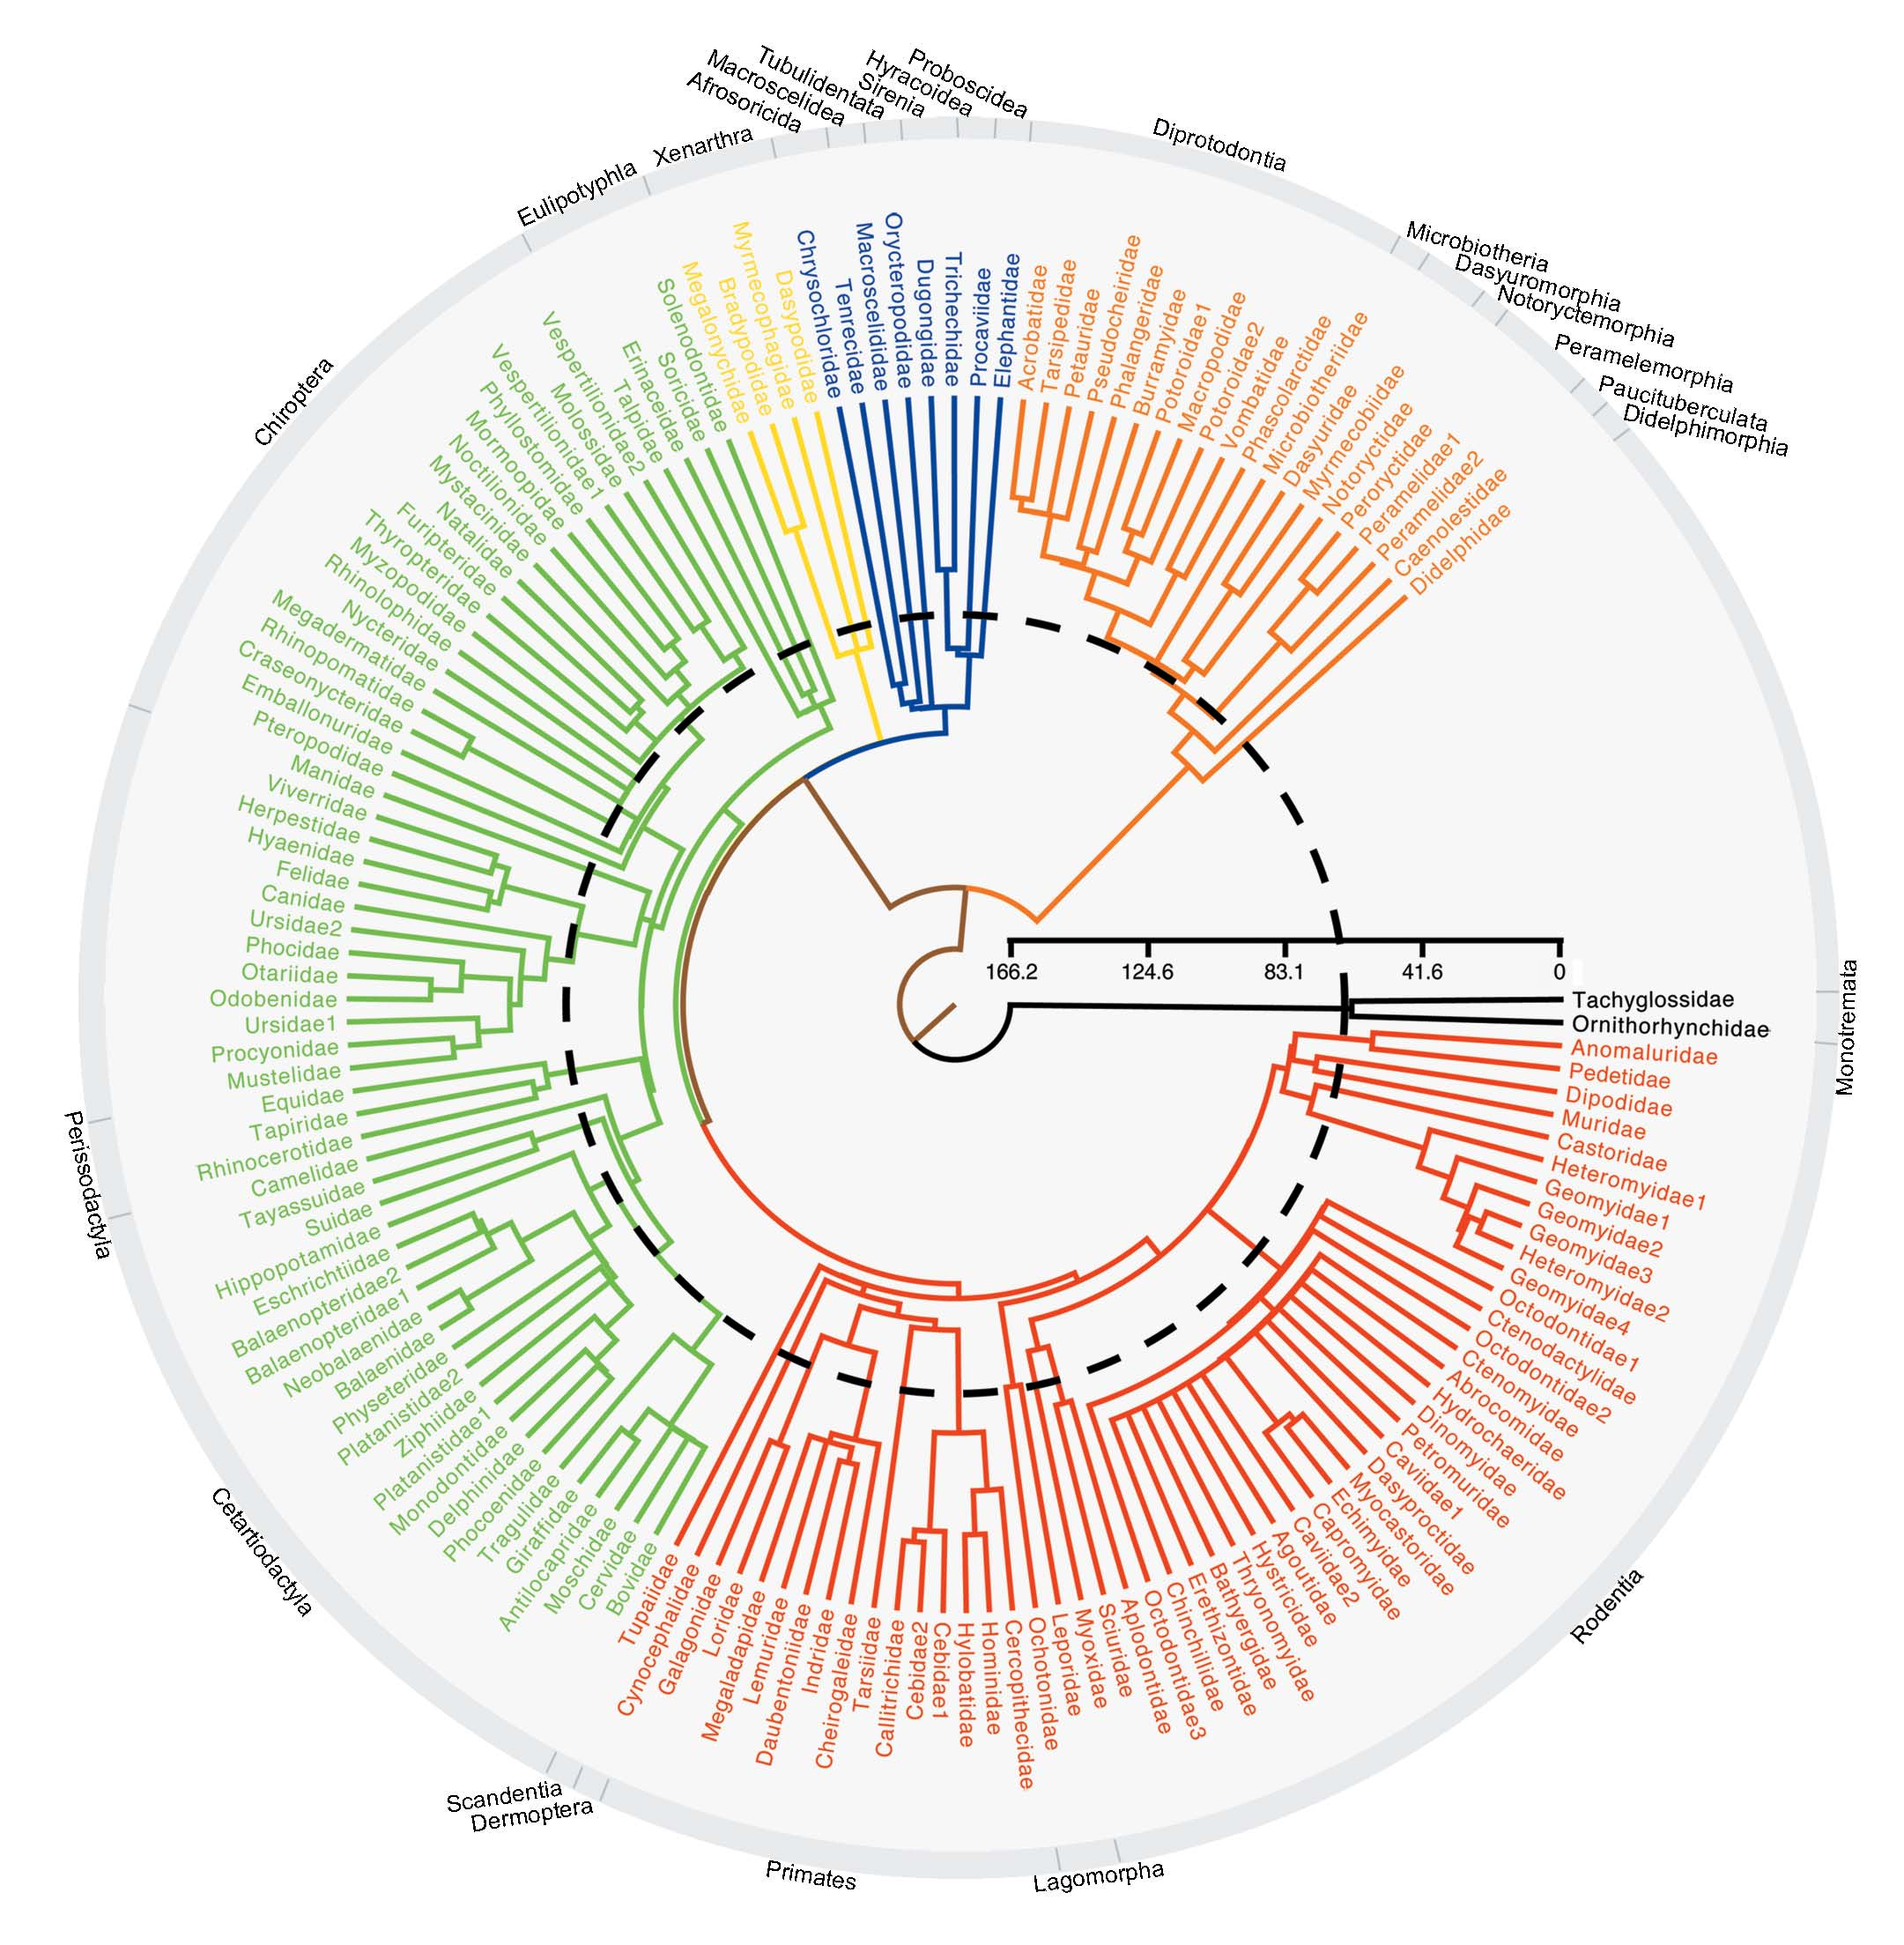
\includegraphics[width=0.40\textwidth]{./images/supertree.bmp}
    \end{columns}
\end{frame}

%%%%%%%%%%%%%%%%%%%%%%%%%%%%%%%%%%%%%%%%%%%%%%%%%%%%%%%%%%%%%%%%%%%%%%%%%%%%%%%%%%%%%%%%%%%%%%%%%%%%%
\begin{frame}{Comprehension of DNA}
\footnotesize
    \begin{columns}[c] % the "c" option specifies center vertical alignment
      \column{.5\textwidth} % column designated by a command
      \begin{itemize}
%       \item They can make \textbf{a whole bacterial genomic map}
      \item They can sequence species ($>5000$ species decoded and listed in \textbf{GenBank})
      \item They can show \textbf{relationship between proteins} of a system (e-Coli)
% % % %       \item They can generate the 3D shape of a protein (fold.It)
      \end{itemize} 
  
      \column{.5\textwidth}
%     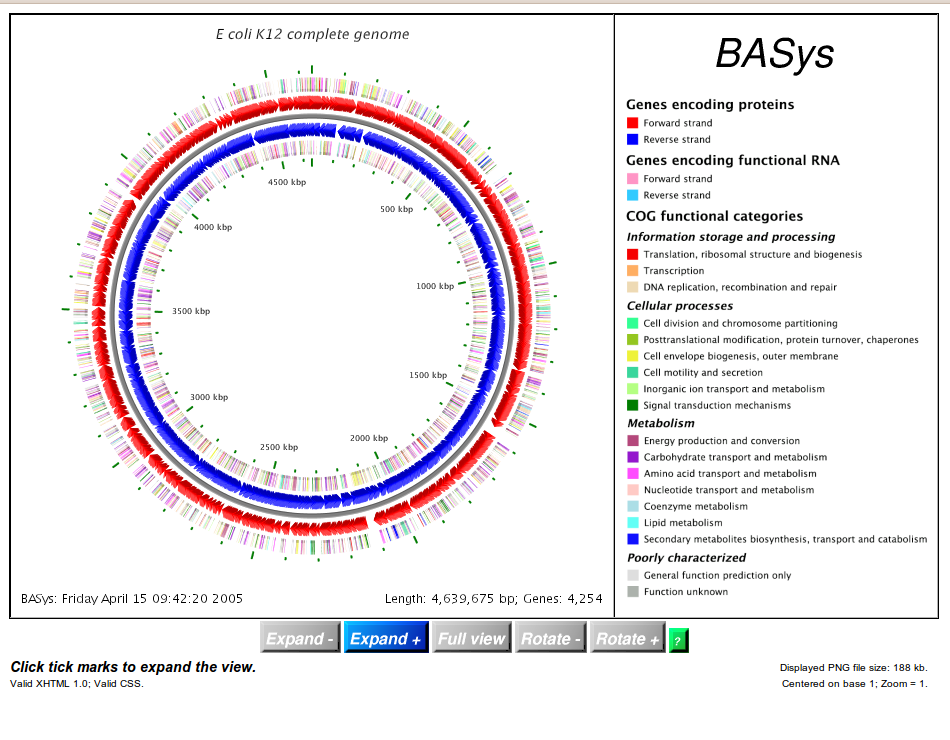
\includegraphics[width=1\textwidth]{./images/BABsys.png} 			
    \includegraphics[width=1.5\textwidth]{./images/supertree2.png}
    \end{columns}
\end{frame}

%%%%%%%%%%%%%%%%%%%%%%%%%%%%%%%%%%%%%%%%%%%%%%%%%%%%%%%%%%%%%%%%%%%%%%%%%%%%%%%%%%%%%%%%%%%%%%%%%%%%%
\begin{frame}{Writing DNA}
\footnotesize
\begin{itemize}
\item To understand it... need to build it
\item early 70’s: start writing our “applications” from scratch (identified enzymes to cut, to glue,... DNA)
\item \textbf{Importance of DNA printers}
  \begin{itemize}
\footnotesize
  \item \textbf{Many DNA manufacturing companies} \\
	(GeneArt, BlueHeron, Medprobe in Oslo, ...)
  \item Really cheap and accessible when: \\ 10 Mbp/hour for $< \$ 100$
  %this will allow to genetically engineer any virtual organism, to build any bacteria from scratch for essentially nothing. (i.e. google toolkit
  \end{itemize}
\end{itemize} 
\end{frame}

%%%%%%%%%%%%%%%%%%%%%%%%%%%%%%%%%%%%%%%%%%%%%%%%%%%%%%%%%%%%%%%%%%%%%%%%%%%%%%%%%%%%%%%%%%%%%%%%%%%%%
\begin{frame}{Writing DNA (Editors/Software)}
\footnotesize
\begin{center}
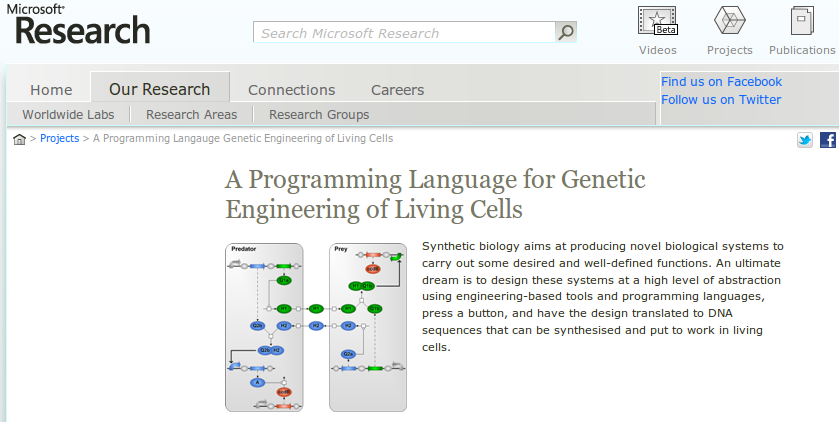
\includegraphics[width=1.0\textwidth]{./images/trueGeneticProgrammingLanguages.png}
\end{center}

\begin{itemize}
\footnotesize
  \item Development of true genetic programming languages 	
  \item debugging “in vitro”
  \item \textbf{“An ultimate dream is to design these systems} %at a high level of abstraction using engineering-based tools and programming languages, 
	  \textbf{press a button, and have the design translated to DNA sequences that can be synthesised 
      and put to work in living cells. ”}
  \end{itemize}
\end{frame}

%%%%%%%%%%%%%%%%%%%%%%%%%%%%%%%%%%%%%%%%%%%%%%%%%%%%%%%%%%%%%%%%%%%%%%%%%%%%%%%%%%%%%%%%%%%%%%%%%%%%%
\begin{frame}{The Human genome coming soon...}
\footnotesize

\begin{center}
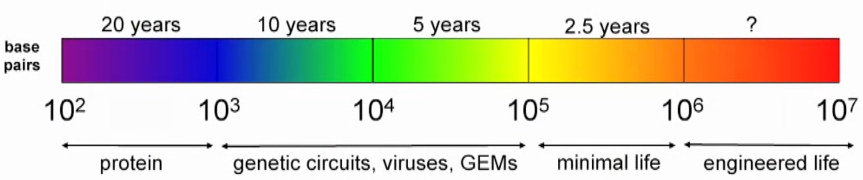
\includegraphics[width=0.8\textwidth]{./images/moreComplexAppsOverTime.jpg}
\end{center}
\begin{center}
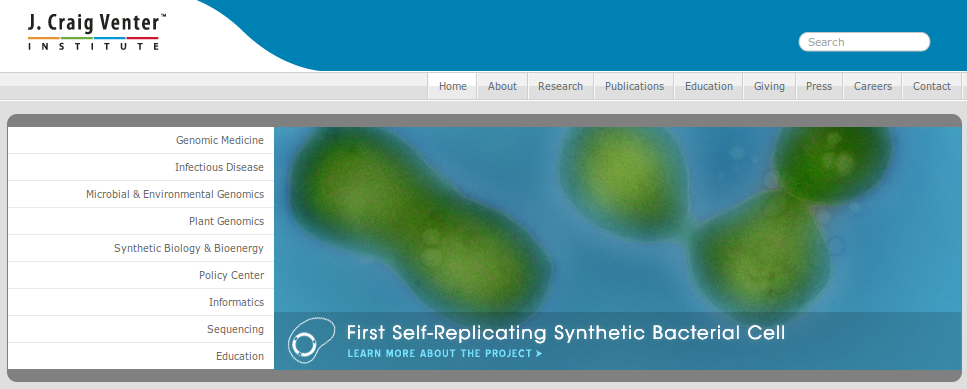
\includegraphics[width=1.0\textwidth]{./images/VenterInstitute.png}
\end{center}
\begin{itemize}
\footnotesize
  \item Quick development of synthetic biology, the next IT industry
  \item The problem today: \textbf{not HOW} to engineer something, but \textbf{for WHAT}! (iGem, Fold.It, DIYBio)
  \end{itemize}
\end{frame}

%%%%%%%%%%%%%%%%%%%%%%%%%%%%%%%%%%%%%%%%%%%%%%%%%%%%%%%%%%%%%%%%%%%%%%%%%%%%%%%%%%%%%%%%%%%%%%%%%%%%%
\begin{frame}{How to contribute?}
\footnotesize
\begin{center}
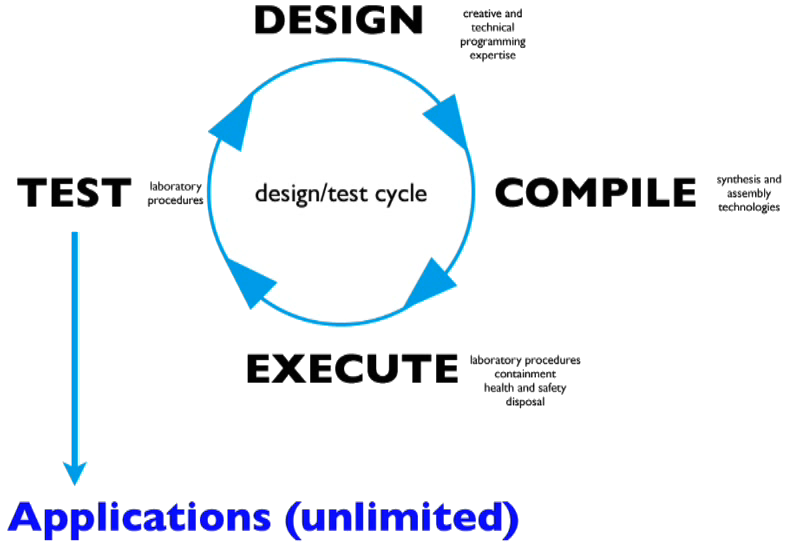
\includegraphics[width=1\textwidth]{./images/wheelOfInnovationWhite.png}
\end{center}
\end{frame}

%%%%%%%%%%%%%%%%%%%%%%%%%%%%%%%%%%%%%%%%%%%%%%%%%%%%%%%%%%%%%%%%%%%%%%%%%%%%%%%%%%%%%%%%%%%%%%%%%%%%%
\begin{frame}{Outline}
\footnotesize
\begin{itemize}
\item What is Synthetic Biology?
\item \textbf{How to computationally design "improved" proteins}
\item What are the challenges for Computational chemistry?
\end{itemize}
\end{frame}


%%%%%%%%%%%%%%%%%%%%%%%%%%%%%%%%%%%%%%%%%%%%%%%%%%%%%%%%%%%%%%%%%%%%%%%%%%%%%%%%%%%%%%%%%%%%%%%%%%%%%
\begin{frame}{Computational protein design algorithms}
\footnotesize
\begin{itemize}
% \item \textbf{homology modeling of proteins} (structure mapping btw structures of target and template proteins)
\item \textbf{Predicting Structure from DNA Sequence?} (from amino acids native conformation)  \\
	\textbf{Not so easy!!!} .The chain can fold up in too many ways! (\textbf{www.Fold.It})
\item \textbf{models of protein energetics} to evaluate how mutations affect the structure and function of proteins 
    \begin{itemize}
\footnotesize
    \item \textbf{molecular mechanics}
    \item \textbf{statistical potential} (i.e. known-proteins in databank)
    \item and other empirical terms
    \end{itemize}

\begin{center}
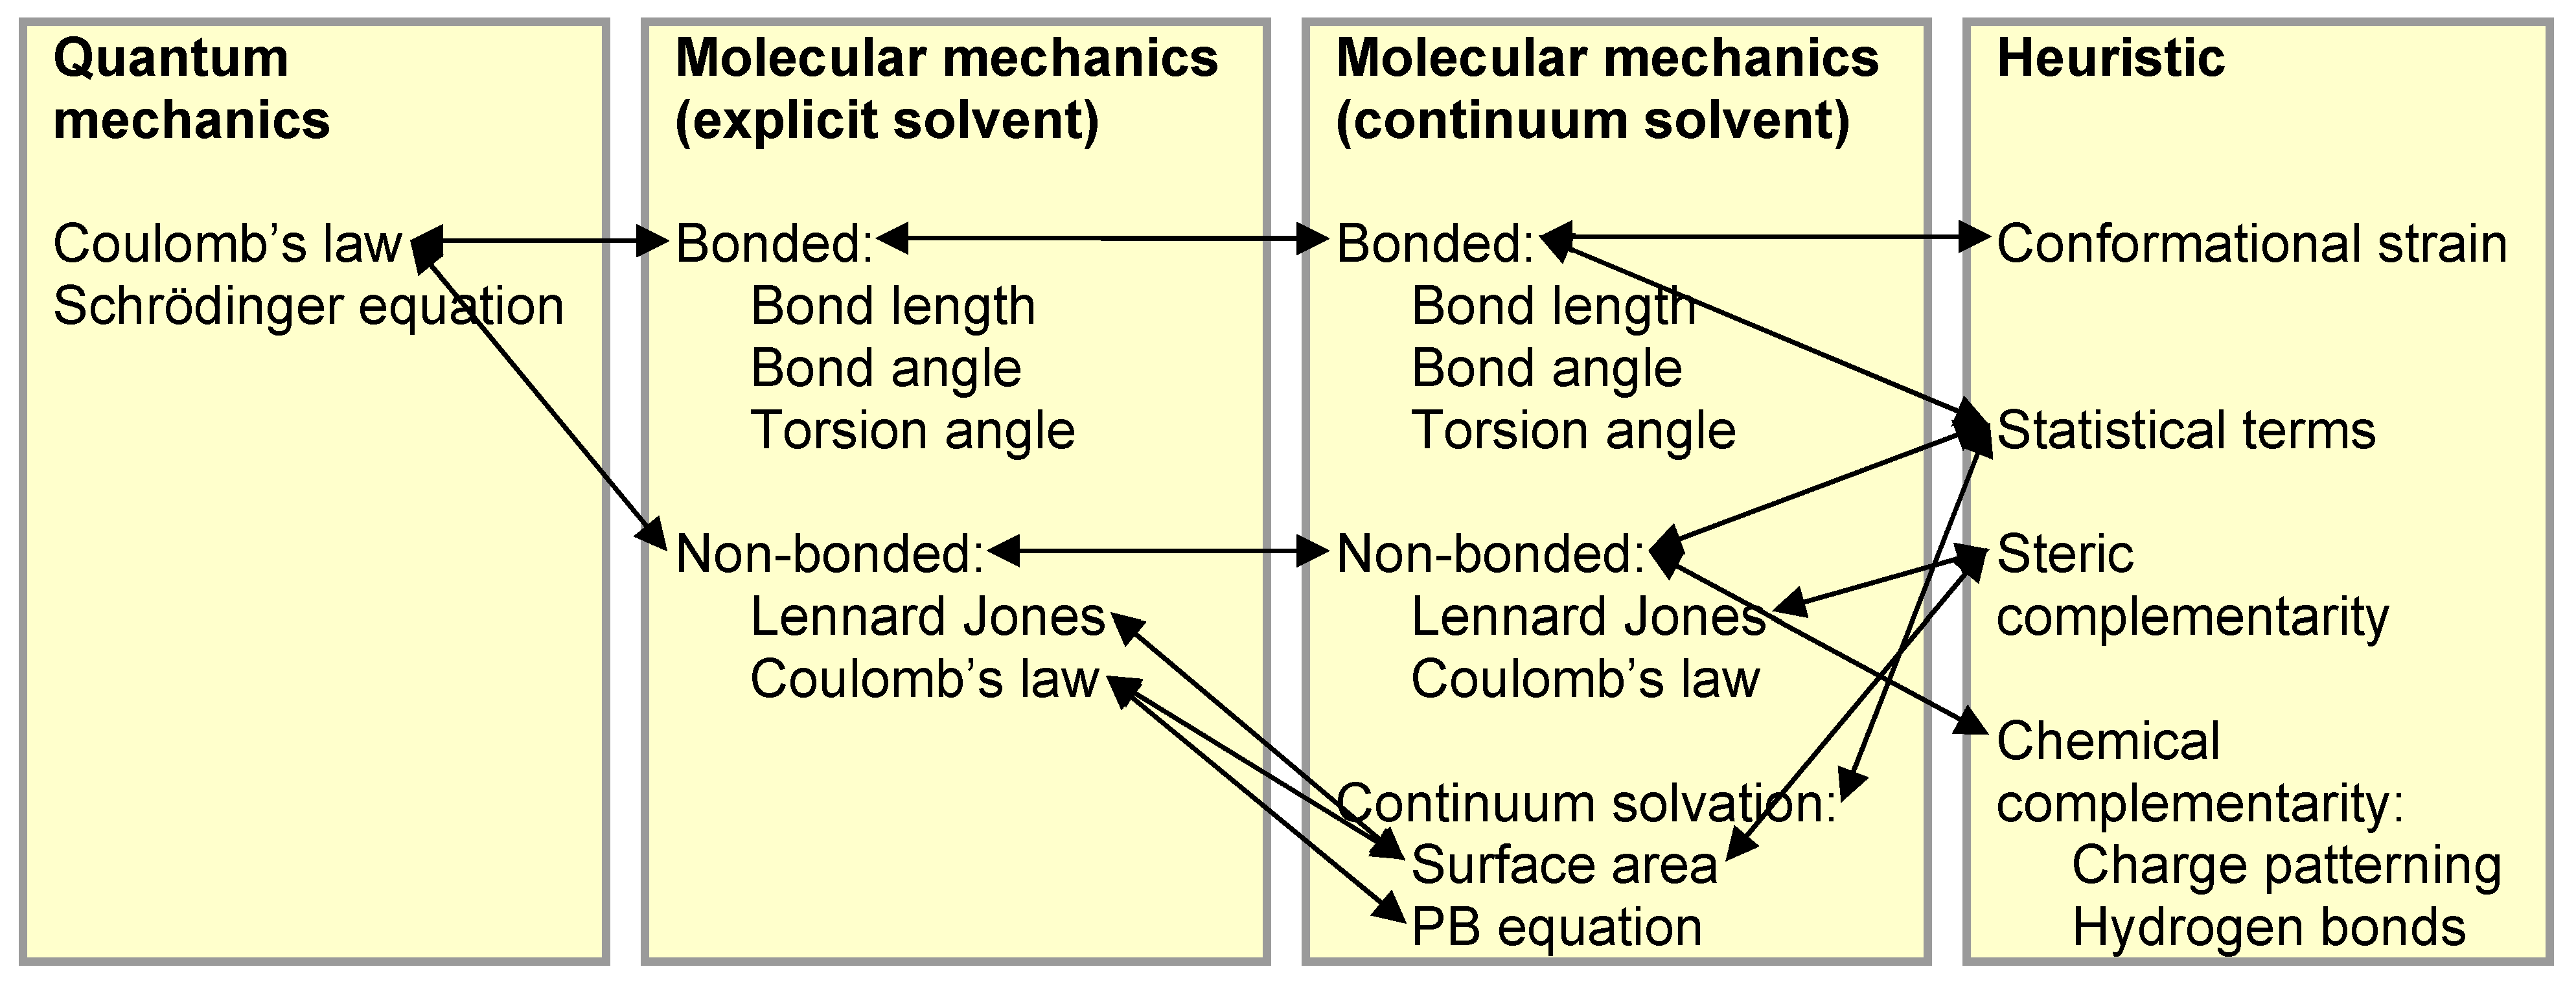
\includegraphics[width=0.8\textwidth]{./images/PEF_comparison.png}
\end{center}
\item  \textbf{QM/MM}
\end{itemize}

\end{frame}


%%%%%%%%%%%%%%%%%%%%%%%%%%%%%%%%%%%%%%%%%%%%%%%%%%%%%%%%%%%%%%%%%%%%%%%%%%%%%%%%%%%%%%%%%%%%%%%%%%%%%
\begin{frame}{Outline}
\footnotesize
\begin{itemize}
\item What is Synthetic Biology?
\item How to computationally design "improved" proteins
\item \textbf{What are the challenges for Computational chemistry?}
\end{itemize}
\end{frame}

%%%%%%%%%%%%%%%%%%%%%%%%%%%%%%%%%%%%%%%%%%%%%%%%%%%%%%%%%%%%%%%%%%%%%%%%%%%%%%%%%%%%%%%%%%%%%%%%%%%
\begin{frame}{Challenges for Computational chemistry: improving designed enzymes}
\footnotesize
\begin{itemize}
% % % \item \textbf{Mechanistic studies}: to identify rate limiting steps in designed enzymes catalyzed reaction
\item \textbf{Structural characterization}: to determine success of active site geometry (e.g. Crystal structures)
\item \textbf{Directed evolution} to identify DNA sequence missing from the design that increases activity 
\item \textbf{Molecular Force Fields}: for better control of side chain conformation, loop conformation, transition state binding orientation.
\item \textbf{Molecular dynamics with explicit solvent}: for assessing conformational stability and population/orientation of transition state in the active site.
\item \textbf{quantum chemistry} and \textbf{QM/MM hybrid methods} in directly determining the magnitude of transition state energy barriers in the context of the designed
active site and ultimately in the context of the designed protein

\end{itemize}
\end{frame}

%%%%%%%%%%%%%%%%%%%%%%%%%%%%%%%%%%%%%%%%%%%%%%%%%%%%%%%%%%%%%%%%%%%%%%%%%%%%%%%%%%%%%%%%%%%%%%%%%%%
\begin{frame}{Summary and Conclusion}
\footnotesize
\begin{itemize}
\item Synthetic Biology: the next IT industry
\item Needs some improvements of the technology to make it accessible to the public 
\item Needs some improvements in identifying and designing "what to improve":  needs \textbf{Computational chemistry}
\end{itemize}
\begin{center}
{\red Thank you for your attention!}
\end{center}
\end{frame}
